\subsection{Mutant Models}

In our final model, we introduce the CLASP protein in order to differentiate the wild type root from the CLASP-1 and BRIN-CLASP mutants. We assume that the CLASP protein $C$ is produced at a basal rate $c_{\text{in}}$. As discussed previously, the BES1 transcription factor inhibits CLASP by repressing its promoter (\cite{ruan2018}, so we include a parameter $c_{B}$ that represents this effect. We also include a background degradation rate $c_{\text{out}}$. Since $C$ will not be fitted to experimental data and is thus dimensionless, we will assign an initial condition of $C(0) = 1$. The differential equation defining the CLASP protein is shown in equation \eqref{clasp}.

\begin{equation}
\label{clasp}
\frac{dC}{dt} = c_{\text{in}} - (c_{\text{out}} + c_{B}\text{BES1})C
\end{equation}

We also need to integrate the two downstream effects of CLASP into our model. It is known that CLASP increases the concentration of BRI1 receptors by promoting their recycling (\cite{ruan2018}). Therefore, we replace the parameter $[\text{BRI1}]$, which was previously fixed to $62\nm$, with equation \eqref{bri1-clasp}. In this equation, $r_{C}$ represents the rate at which CLASP promotes the recycling of $[\text{BRI1}]$ receptors while $r_{P}$ denotes the basal receptor level in the abscence of CLASP.

\begin{equation}
\label{bri1-clasp}
[\text{BRI1}] = R_{T} = r_{C}C + r_{P}
\end{equation}

Experiments have also found that CLASP inhibits growth in a length-dependent manner. Therefore, we add a $g_{C}C / L$ term to the denominator of  equation \eqref{growth} to get the modified version shown in equation \eqref{growth-clasp}. We also omit the $g_{P}$ parameter used in equation \eqref{growth} because this parameter was fit to effectively $0$ in Figure \ref{fig:growth-model-fit}.

\begin{equation}
\label{growth-clasp}
\frac{dL}{dt} = \frac{g_{B}\text{BES1}}{1 + (g_{C}C/L)}
\end{equation}

An overview of the entire model incorporating BL, BRI1, BES1, CLASP, and cell growth is presented in Figure \ref{fig:clasp-model}. The differential equations used in the model were approximated using a forward euler method with time step $0.01\h$. The model accuracy was quantified using the sum of the RMSE from each dataset (Wild Type, CLASP-1, BRIN-CLASP). In CLASP-1 roots we fixed the parameter values $c_{\text{in}} = c_{\text{out}} = c_{B} = 0$. For the BRIN-CLASP root we set $c_{B} = 0$. All other parameters were held constant accross the three mutants.

\begin{figure}
    \centering
    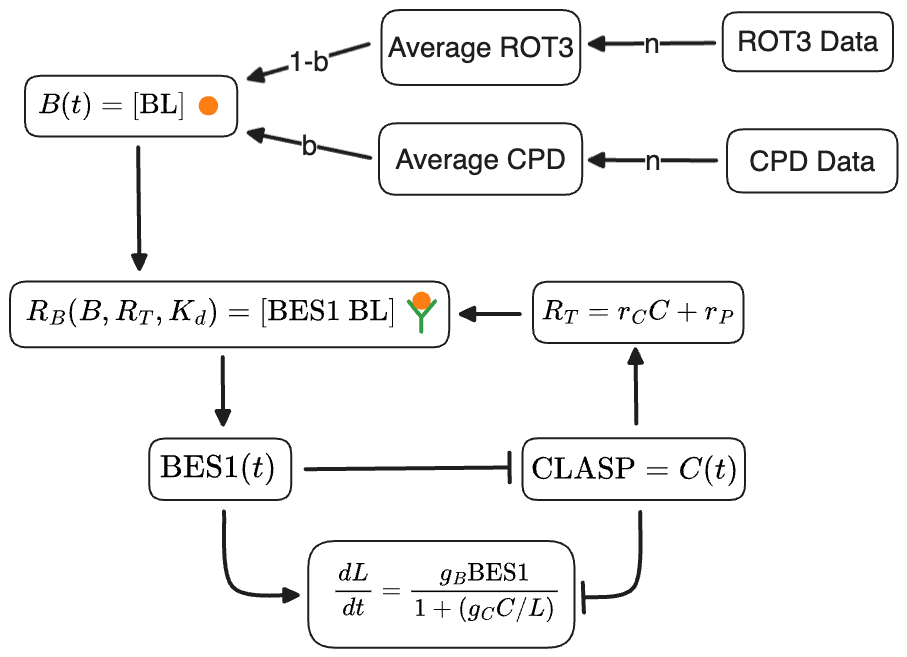
\includegraphics[width=13cm]{img/clasp-model.png}
    \caption{Our complete model of cell growth in \emph{A. thaliana} which contains the BL concentration $B$, the BRI1 concentration $R_{T}$, the bound receptor concentration $R_{B}$, the level of $\text{BES1}$ signalling, the quantity of CLASP protein $C$, and the length of the cell $L$.}
    \label{fig:clasp-model}
\end{figure}


